\documentclass{amsart}

%\documentclass{amsart}
\usepackage[utf8]{inputenc}
\usepackage{amsfonts}
\usepackage{amsmath}
\usepackage{amssymb}
\usepackage{amsthm}
\usepackage{asymptote}
\usepackage{mathtools}
\usepackage{hhline}
\usepackage{graphicx,enumerate}
\usepackage{hyperref}
\usepackage[a4paper, margin=1.2in]{geometry}
%\usepackage{tcolorbox}
\usepackage{tikz-cd}
\usepackage{ytableau}
%\tcbuselibrary{skins,breakable,xparse}
\allowdisplaybreaks
\newcounter{count}
\hypersetup{
	colorlinks=true,
	linkcolor=teal,
	filecolor=magenta,      
	urlcolor=olive,
	citecolor=teal,
	pdfpagemode=FullScreen,
}

%\definecolor{defcolor}{HTML}{478EFF}
%\definecolor{thmcolor}{HTML}{CC0058}
%\definecolor{excolor}{HTML}{F5B400}
%\definecolor{probcolor}{HTML}{DD4803}
%\definecolor{lemcolor}{HTML}{741FEA}
%\definecolor{scarlet}{HTML}{A81111}
%
%\newtheoremstyle{definitionStyle}% Custom style for definitions
%{0.5em}% Space above
%{0.5em}% Space below
%{}% Body font
%{}% Indent amount
%{\bfseries\color{defcolor}}% Theorem head font: bold and red
%{.\\}% Punctuation after theorem head
%{0.5em}% Space after theorem head
%{\thmname{#1}\thmnumber{ #2 (#3)}}% Theorem head spec
%
%\theoremstyle{definitionStyle}
%\newtheorem{df}{Definition}[section]
%
%\newtheoremstyle{theoremStyle}% Custom style for definitions
%{0.5em}% Space above
%{0.5em}% Space below
%{}% Body font
%{}% Indent amount
%{\bfseries\color{thmcolor}}% Theorem head font: bold and red
%{.\\}% Punctuation after theorem head
%{0.5em}% Space after theorem head
%{\thmname{#1}\thmnumber{ #2 (#3)}}% Theorem head spec
%
%\theoremstyle{theoremStyle}
%\newtheorem{thm}{Theorem}[section]
%
%\newtheoremstyle{lemmaStyle}% Custom style for definitions
%{0.5em}% Space above
%{0.5em}% Space below
%{}% Body font
%{}% Indent amount
%{\bfseries\color{lemcolor}}% Theorem head font: bold and red
%{.\\}% Punctuation after theorem head
%{0.5em}% Space after theorem head
%{\thmname{#1}\thmnumber{ #2 (#3)}}% Theorem head spec
%
%\theoremstyle{lemmaStyle}
%\newtheorem{lem}{Lemma}[section]
%\newtheorem{cor}{Corollary}[section]
%
%\newtheoremstyle{exampleStyle}% Custom style for definitions
%{0.5em}% Space above
%{0.5em}% Space below
%{}% Body font
%{}% Indent amount
%{\bfseries\color{excolor}}% Theorem head font: bold and red
%{.\\}% Punctuation after theorem head
%{0.5em}% Space after theorem head
%{\thmname{#1}\thmnumber{ #2 (#3)}}% Theorem head spec
%
%\theoremstyle{exampleStyle}
%\newtheorem{ex}{Example}[section]
%
%\newtheoremstyle{problemStyle}% Custom style for definitions
%{0.5em}% Space above
%{0.5em}% Space below
%{}% Body font
%{}% Indent amount
%{\bfseries\color{probcolor}}% Theorem head font: bold and red
%{.\\}% Punctuation after theorem head
%{0.5em}% Space after theorem head
%{\thmname{#1}\thmnumber{ #2#3}}% Theorem head spec
%
%\theoremstyle{problemStyle}
%\newtheorem{prob}{Problem}[section]

% For Fun
\newcommand{\club}{\color{teal} \clubsuit}
\newcommand{\heart}{\color{red} \heartsuit}
\renewcommand{\star}{\color{scarlet} \bigstar}
\newcommand{\spade}{\color{violet} \spadesuit}

% Symbols
\newcommand{\A}{\mathcal{A}}
\newcommand{\B}{\mathcal{B}}
\newcommand{\C}{\mathbb{C}}
\newcommand{\D}{\mathcal{D}}
\newcommand{\E}{\mathbb{E}}
\newcommand{\F}{\mathbb{F}}
\newcommand{\G}{\mathcal{G}}
% \renewcommand{\H}{\mathcal{H}} Erdos o
\newcommand{\I}{\mathcal{I}}
\newcommand{\J}{\mathcal{J}}
\newcommand{\K}{\mathcal{K}}
% \renewcommand{\L}{\mathcal{L}}
\newcommand{\M}{\mathcal{M}}
\newcommand{\N}{\mathbb{N}}
\renewcommand{\O}{\mathcal{O}}
\renewcommand{\P}{\mathbb{P}}
\newcommand{\Q}{\mathbb{Q}}
\newcommand{\R}{\mathbb{R}}
\renewcommand{\S}{\mathbb{S}}
\newcommand{\T}{\mathbb{T}}
\newcommand{\U}{\mathcal{U}}
\newcommand{\V}{\mathcal{V}}
\newcommand{\W}{\mathcal{W}}
\newcommand{\X}{\mathcal{X}}
\newcommand{\Y}{\mathcal{Y}}
\newcommand{\Z}{\mathbb{Z}}

\renewcommand{\AA}{\mathcal{A}}
\newcommand{\BB}{\mathcal{B}}
\newcommand{\CC}{\mathcal{C}}
\newcommand{\DD}{\mathcal{D}}
\newcommand{\EE}{\mathcal{E}}
\newcommand{\FF}{\mathcal{F}}
\newcommand{\GG}{\mathbb{G}}
\newcommand{\HH}{\mathbb{H}}
\newcommand{\calH}{\mathcal{H}}
\newcommand{\II}{\mathcal{I}}
\newcommand{\JJ}{\mathcal{J}}
\newcommand{\KK}{\mathcal{K}}
\newcommand{\LL}{\mathcal{L}}
\newcommand{\MM}{\mathcal{M}}
\newcommand{\NN}{\mathcal{N}}
\newcommand{\OO}{\mathrm{O}}
\newcommand{\PP}{\mathcal{P}}
\newcommand{\QQ}{\mathcal{Q}}
\newcommand{\RR}{\mathcal{R}}
\renewcommand{\SS}{\mathcal{S}}
\newcommand{\TT}{\mathcal{T}}
\newcommand{\UU}{\mathcal{U}}
\newcommand{\VV}{\mathcal{V}}
\newcommand{\WW}{\mathcal{W}}
\newcommand{\XX}{\mathcal{X}}
\newcommand{\YY}{\mathcal{Y}}
\newcommand{\ZZ}{\mathcal{Z}}
\renewcommand{\d}{\textrm{d}}
% Greek letters
\newcommand{\ep}{\varepsilon}
\newcommand{\ph}{\varphi}
\newcommand{\de}{\delta}
\renewcommand{\a}{\alpha}
\renewcommand{\b}{\beta}
% Fraktur
\newcommand{\mm}{\mathfrak{m}}
\renewcommand{\aa}{\mathfrak{a}}
\newcommand{\bb}{\mathfrak{b}}
\newcommand{\pp}{\mathfrak{p}}
\newcommand{\qq}{\mathfrak{q}}
% Operators
\DeclareMathOperator{\Div}{div}
\DeclareMathOperator{\Gal}{Gal}
\DeclareMathOperator{\vol}{Vol}
\DeclareMathOperator{\Hom}{Hom}
\DeclareMathOperator{\End}{End}
\DeclareMathOperator{\Ext}{Ext}
\DeclareMathOperator{\Tor}{Tor}
\DeclareMathOperator{\tr}{tr}
\DeclareMathOperator{\rk}{rk}
\DeclareMathOperator{\curl}{curl}
\DeclareMathOperator{\mesh}{mesh}
\DeclareMathOperator{\im}{im}
\DeclareMathOperator{\coker}{coker}
\DeclareMathOperator{\width}{width}
\DeclareMathOperator{\diam}{diam}
\DeclareMathOperator{\maps}{Maps}
\DeclareMathOperator{\Frac}{Frac}
\DeclareMathOperator{\Sym}{Sym}
\DeclareMathOperator{\sgn}{sgn}
\DeclareMathOperator{\alt}{Alt}
\DeclareMathOperator{\supp}{supp}
\DeclareMathOperator{\Span}{span}
\DeclareMathOperator{\Var}{Var}
\DeclareMathOperator{\Spec}{Spec}

\newcommand{\nor}{\unlhd}
\DeclareMathOperator{\aut}{Aut}
\DeclareMathOperator{\orb}{Orb}
\DeclareMathOperator{\GL}{GL}
\DeclareMathOperator{\SL}{SL}
\DeclareMathOperator{\SO}{SO}
\DeclareMathOperator{\PGL}{PGL}
\DeclareMathOperator{\PSL}{PSL}
\DeclareMathOperator{\stab}{Stab}
\DeclareMathOperator{\fix}{Fix}
\DeclareMathOperator{\Th}{Th}
\DeclareMathOperator{\Ind}{Ind}
\DeclareMathOperator{\Res}{Res}
\DeclareMathOperator{\Ann}{Ann}
\DeclareMathOperator{\rad}{rad}
\DeclareMathOperator{\len}{len}
\DeclareMathOperator{\ord}{ord}

% \DeclareMathOperator{\arg}{arg}

%% misc
\newcommand{\<}{\langle}
\renewcommand{\>}{\rangle}
\renewcommand{\^}{\wedge}
\renewcommand{\v}{\vee}
\def\Xint#1{\mathchoice
	{\XXint\displaystyle\textstyle{#1}}%
	{\XXint\textstyle\scriptstyle{#1}}%
	{\XXint\scriptstyle\scriptscriptstyle{#1}}%
	{\XXint\scriptscriptstyle\scriptscriptstyle{#1}}%
	\!\int}
\def\XXint#1#2#3{{\setbox0=\hbox{$#1{#2#3}{\int}$ }
		\vcenter{\hbox{$#2#3$ }}\kern-.6\wd0}}
\def\ddashint{\Xint=}
\def\dashint{\Xint-}
%% arrows
\newcommand{\xhra}{\xhookrightarrow}
\newcommand{\xra}{\xrightarrow}
\newcommand{\ra}{\rightarrow}
\newcommand{\rra}{\rightrightarrows}
\newcommand{\lra}{\longrightarrow}
\newcommand{\Ra}{\Rightarrow}
\newcommand{\lRa}{\Longrightarrow}
\newcommand{\lrsa}{\leftrightsquiqarrow}
\newcommand{\ba}{\leftrightarrow}
%% lists
\newcommand{\be}{\begin{enumerate}[(i)]}
	\newcommand{\ee}{\end{enumerate}}
%% integration stuff
\newcommand{\calR}{\mathcal{R}}
\newcommand{\rint}{\calR\!\int}
\newcommand{\calL}{\mathcal{L}}
\newcommand{\lowerint}{\mbox{\b{$\int$}}}
\newcommand{\upperint}{{\textstyle\bar{\int}}}
%% end of proof
\def\endproof{{\hfill $\Box$}}
%% matrix shorthand

\title{Math 317 HW 3}
\author{Jalen Chrysos}

\begin{document}
	\maketitle

\textbf{Problem 1 (Hatcher 1.2:9)}: In the surface $M_g$ of genus $g$, let $C$ be a circle that separates $M_g$ into two compact surfaces $M_h'$ and $M_k'$ obtained from the closed surfaces $M_h$ and $M_k$ by deleting an open disk from each. Show that $M_h'$ does not retract onto $C$, and hence $M_g$ does not retract onto $C$. But show that $M_g$ does retract onto the non-separating circle $C'$ in the figure.

\begin{center}
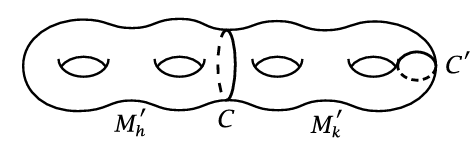
\includegraphics[height=3cm]{"C:/Users/jzchr/MathDocuments/Class Work/Topology/Homework/317HW3/Fig_1.9_Hatcher.png"}
\end{center}

\begin{proof}
	If there is any retraction $r:M_h'\to C$, then this $r$ induces a map of the first homology groups $r_*$. Composing $r$ with the inclusion $\iota:C\to M_h'$, induces the identity on $H_1(C)=\Z$:
	$$
	H_1(C)\xrightarrow{\iota_*} H_1(M_h')\xra{r_*} H_1(C)
	$$
	Now we will show that $\id_{\Z}$ cannot factor through $H_1(M_h')$:\\
	
	We know that $H_1(M_h)$ can be presented as the Abelianization of
	$$
	\pi_1(M_h) = \<a_1,b_1,a_2,b_2,\dots,a_h,b_h \; | \; [a_1,b_1][a_2,b_2]\cdots [a_h,b_h]\>,
	$$
	which is $\Z^{2h}$. For $M_h'$, things are different because there is a puncture, which we can represent as an additional loop $c$ at one of the vertices, so rather than the product of commutators being a loop, it is just equal to $c$; that is,
	$$
	\pi_1(M_h') = \<a_1,b_1,\dots,a_h,b_h,c \; | \; [a_1,b_1]\cdots[a_h,b_h] = c\>
	$$
	so $H_1(M_h')$ is the Abelianization of this. The image $\iota_*(1)\in \pi_1(M_h')$ is exactly the loop $c$, but this $c$ is 0 in $H_1(M_h')$, so $\iota_*$ is trivial on the homology groups, and thus $r_*\circ \iota_*$ cannot be the identity. So $r$ cannot exist in the first place.\\
%	Since $\pi_1(C)=\Z$ is Abelian, $r_*(\Z)$ will have to be Abelian in $\pi_1(M_h')$, i.e. the image is inside the Abelianization, in which all the commutators and $c$ are trivial. But $C$ includes as the loop $c$, so $r_*(\pi_1(C))=0$, and thus $r_*\circ \iota_*$ cannot be the identity, so $r_*$ cannot exist.\\
	
	On the other hand, $C'$ corresponds to one of the sides of the $2g$-gon, not an additional loop, so the argument does not work for $C'$. And it is possible to retract to $C'$ by multiple methods. For one, you can fold up the $2g$-gon along the long diagonals repeatedly until left with four edges corresponding to one commutator (i.e. a single torus). Then with this torus, just project down onto one of the sides of the square.
\end{proof}

\newpage
\textbf{Problem 2 (Hatcher 1.2:11)}: The mapping torus $T_f$ of a map $f:X\to X$ is the quotient of $X\times I$ obtained by identifying each point $(x,0)$ with $(f(x),1)$. In the case $X=S^1\vee S^1$ with $f$ preserving the basepoint, compute a presentation for $\pi_1(T_f)$ in terms of the induced map $f_*:\pi_1(X)\to\pi_1(X)$. Do the same when $X=S^1\times S^1$.
\begin{proof}
	$T_f$ has a CW-complex construction with a single 0-cell $x$, two 1-cells $\a$ and $\b$, and two 2-cells which attach via $f$, giving the relations $\a = f_*(\a)$ and $\b=f_*(\b)$. So the group presentation is 
	$$
	\pi_1(T_f) = \<\a,\b \; | \; \a = f_*(\a),\; \b = f_*(\b)\>.
	$$
	When $X=S^1\times S^1$, we start with the free abelian group on two generators $\Z^2$ and again identify $\a=f_*(\a)$ and $\b=f_*(\b)$, giving
	$$
	\pi_1(T_f) = \<\a,\b \; | \; \a = f_*(\a), \; \b = f_*(\b), \; \a\b=\b\a \>.
	$$
\end{proof}

\newpage
\textbf{Problem 3 (Hatcher 1.2:14)}: Consider the quotient space $X$ of a cube $I^3$ obtained by identifying each square face with the opposite square face via a clockwise quarter-rotation and translation by one unit. Show that $X$ is a cell complex with two $0$-cells, four $1$-cells, three $2$-cells, and one $3$-cell. Using this structure, show that $\pi_1(X)$ is the quaternion group.
\begin{proof}
	The cells are as in the diagram. The two 0-cells are denoted by black and white circles, which are identified. The four 1-cells are the arrows $a,b,c,d$. The three 2-cells are the faces of the cube (with opposite faces identified by quarter turn). The single 3-cell is the cube itself.
	$$
	\begin{tikzcd}
		&& \bullet \\
		\circ &&&&& \circ \\
		&&& \bullet \\
		&& \circ \\
		\bullet &&&&& \bullet \\
		&&& \circ
		\arrow["c"{description}, color={rgb,255:red,92;green,214;blue,214}, from=1-3, to=2-1]
		\arrow["d"{description}, color={rgb,255:red,92;green,214;blue,92}, from=1-3, to=2-6]
		\arrow["a"{description, pos=0.3}, color={rgb,255:red,214;green,92;blue,92}, from=1-3, to=4-3]
		\arrow["b"{description}, color={rgb,255:red,92;green,92;blue,214}, from=3-4, to=2-1]
		\arrow["a"{description}, color={rgb,255:red,214;green,92;blue,92}, from=3-4, to=2-6]
		\arrow["c"{description, pos=0.3}, color={rgb,255:red,92;green,214;blue,214}, from=3-4, to=6-4]
		\arrow["d"{description}, color={rgb,255:red,92;green,214;blue,92}, from=5-1, to=2-1]
		\arrow["b"{description}, color={rgb,255:red,92;green,92;blue,214}, from=5-1, to=4-3]
		\arrow["a"{description}, color={rgb,255:red,214;green,92;blue,92}, from=5-1, to=6-4]
		\arrow["b"{description}, color={rgb,255:red,92;green,92;blue,214}, from=5-6, to=2-6]
		\arrow["c"{description}, color={rgb,255:red,92;green,214;blue,214}, from=5-6, to=4-3]
		\arrow["d"{description}, color={rgb,255:red,92;green,214;blue,92}, from=5-6, to=6-4]
	\end{tikzcd}
	$$
	
	In the 1-skeleton, $X^1$ has 4 edges $a,b,c,d$. The fundamental group $\pi_1(X^1)$ is generated by 
	$$
	i := ab^{-1}, \; j := ac^{-1}, \; k = ad^{-1}.
	$$
	The attaching maps of the three 2-cells yield the relations
	$$
	ad^{-1}bc^{-1} = 1, \;\; ac^{-1}db^{-1}=1, \;\; ab^{-1}cd^{-1} = 1.
	$$
	Translating this to $i,j,k$, we can say $j = ac^{-1} = bd^{-1} = ba^{-1}ad^{-1} = i^{-1}k \Rightarrow ij = k$. Likewise,
	$$
	i = jk, \;\; j = ki, \;\; k = ij.
	$$
	And we also have 
	\begin{align*}
		kji &= (ad^{-1})ac^{-1}ab^{-1}\\
		&= c(b^{-1}ac^{-1})ab^{-1}\\
		&= cd^{-1}ab^{-1}\\
		&= 1
	\end{align*}
	(this can be seen as a deformation of the loop in the diagram). Thus, $i,j,k$ obey the group presentation for $Q$: note that
	$$
	i^2 = ijk = k^2 = kij = j^2
	$$
	and 
	$$
	(ijk)^2 = (ij)(ki)(jk) = kji = 1.
	$$
\end{proof}

\newpage 
\textbf{Problem 4 (Hatcher 1.2:16)}: Show that the fundamental group of the surface of infinite genus is free on an infinite number of generators.
\begin{proof}
	Similarly to the surfaces of finite genus, we can give a CW complex structure to the surface $M_{\omega}^+$ with infinite genus \textit{in one direction}: one 0-cell $x$, infinitely many 1-cells $a_1,b_1,a_2,b_2,\dots$, and a single 2-cell which attaches via $$a_1b_1a_1^{-1}b_1^{-1}a_2b_2a_2^{-1}b_2^{-1}\cdots$$
	This makes $\pi_1(M_{\omega}^+)=\Z^{\omega}$, as this infinite product of commutators is not actually a group element.\\
	
	Now to get the fundamental group of $M_{\omega}$, which has infinitely many holes extending in both directions: we can write $M_{\omega}\simeq M_{\omega}^+\vee M_{\omega}^+$, so by Van Kampen's Theorem,
	$$\pi_1(M_{\omega})=\Z^{\omega}\oplus \Z^{\omega} = \Z^{\omega+\omega} = \Z^{\omega}.$$
\end{proof}

\newpage
\textbf{Problem 5 (Hatcher 1.2:22)}: In this exercise, we describe an algorithm for computing the \textit{Wirtinger presentation} of the fundamental group of the complement of a knot in $\R^3$. We begin with the knot lying almost flat on a table $T$ so that $K$ consists of finitely-many disjoint arcs $\a_i$ contained within $T$ and finitely-many $\b_{\ell}$ which leave $T$ to cross over another part of $K$. We build a 2-dimensional complex $X$ that is a deformation retract of $\R^3-K$ by taking $X$ to essentially be a tube that surrounds the string and contacts itself when there is a crossing:\\

For each $\a_i$, let $R_i$ be a curved rectangle so that its long edges are on $T$ and it has $\a_i$ underneath it, and let and $\b_{\ell}$ crossing over $\a_i$ lie along the curve of $R_i$. For each $\b_{\ell}$, let $S_{\ell}$ be the square-shaped piece which covers the crossing, so that $\b_{\ell}$ lies under $S_{\ell}$ but inside $R_i$. Let $X$ be the union of $T$, $R_i$, and $S_{\ell}$ for all $i,\ell$. Lift $K$ off the table slightly so that it does not intersect $X$. Then we can deformation retract $\R^3-K$ to $X$.\\

\begin{enumerate}[(a)]
	\item Assuming that this retraction is possible, show that $\pi_1(\R^3-K)$ has a presentation with one generator $x_i$ for each $R_i$ and one relation $x_ix_jx_i^{-1}=x_k$ whenever $\a_j,\a_k$ are two pieces which cross over $\a_i$ via some $\b_{\ell}$.
	\item Use this presentation to show that the Abelianization of $\pi_1(\R^3-K)$ is $\Z$.
\end{enumerate}
\begin{proof}
	(a): By the deformation retraction, $\pi_1(\R^3-K)=\pi_1(X)$. $X$ can be constructed as a CW complex with 1-cells $x_i$ corresponding to the arcs where $\a_i$ meets the square $S_{\ell}$, and 2-cells forming the tubes (note that this makes the arcs at the beginning and end of tube $\a_i$ \textit{both} equivalent to $x_i$) and the identifications given by each crossing square $S_{\ell}$. Traversing around a crossing counterclockwise (or clockwise, as long as it's consistent), the attaching map gives $x_ix_jx_i^{-1}x_k^{-1}$, so by Van Kampen's theorem we quotient by this relation to get the correct group presentation.\\
	
	(b): In the Abelianization of $\pi_1(X)$, $x_ix_jx_i^{-1}=x_j$, so this gives $x_k=x_j$ for all $k,j$ that are separated by a crossing. But since $K$ is a knot in the first place, all of the segments are related this way. So $\pi_1(X)$ has a single generator with no relations, i.e. it is $\Z$.
\end{proof}

\newpage
\textbf{Problem 6 (Hatcher 1.B:5)}: Consider the graph of groups $\Gamma$ having one vertex $\Z$ and one edge $n\mapsto 2n$. Show that $\pi_1(K\Gamma)$ has presentation $\<a,b\;|\;bab^{-1}a^{-2}\>$ and describe the universal cover of $K\Gamma$ explicitly as a product $T\times \R$ with $T$ a tree.
\begin{proof}
	$K\Gamma$ consists of $S^1$ along with a mapping cylinder which attaches $x$ to $2x$. Thus we have the CW complex presentation below:
	$$
	\begin{tikzcd}
		&& X \\
		& \bullet && \bullet \\
		{[0,1]} \\
		& \bullet & \bullet & \bullet
		\arrow["a", from=2-2, to=2-4]
		\arrow["b"', two heads, from=2-2, to=4-2]
		\arrow["b", two heads, from=2-4, to=4-4]
		\arrow["a"', from=4-2, to=4-3]
		\arrow["a"', from=4-3, to=4-4]
	\end{tikzcd}
	$$
	All the black dots are identified and the similarly labeled arrows are identified. $a$ represents a single loop in $S^1$ and $b$ the loop around the mapping cylinder (it's really more of a mapping torus in this case). We can see that the single relation given by the 2-cell is $aba^{-2}b^{-1}=1$, giving the desired group presentation.\\

	In the universal cover, we want to tile some 2-dimensional surface with these squares so that every point is the corner of two squares of sidelength $x$ and two more of sidelength $2x$ (because they are identified with the vertices on the bottom). This forces the two top vertices to be connected to \textit{separate} squares of sidelength $2x$, since they cannot both fit. Thus at the top of each square we have to split into two, and so on. This creates an infinite 3-valent tree $T$ in one direction, and just a non-branching $\R$ in the other. So the universal cover is $T\times \R$.
	
	Below is a depiction of the splitting at one of the nodes of $T$:
	$$
	\begin{tikzcd}
		& \bullet && \bullet && \bullet && \bullet \\
		\\
		\cdots & \bullet & \bullet & \bullet & \bullet & \bullet & \bullet & \bullet & \bullet & \cdots \\
		\\
		&& \bullet && \bullet && \bullet && \bullet
		\arrow[from=1-2, to=1-4]
		\arrow[two heads, from=1-2, to=3-2]
		\arrow[from=1-4, to=1-6]
		\arrow[two heads, from=1-4, to=3-4]
		\arrow[from=1-6, to=1-8]
		\arrow[two heads, from=1-6, to=3-6]
		\arrow[two heads, from=1-8, to=3-8]
		\arrow[from=3-1, to=3-2]
		\arrow[from=3-2, to=3-3]
		\arrow[from=3-3, to=3-4]
		\arrow[from=3-4, to=3-5]
		\arrow[from=3-5, to=3-6]
		\arrow[from=3-6, to=3-7]
		\arrow[from=3-7, to=3-8]
		\arrow[from=3-8, to=3-9]
		\arrow[from=3-9, to=3-10]
		\arrow[two heads, from=5-3, to=3-3]
		\arrow[from=5-3, to=5-5]
		\arrow[two heads, from=5-5, to=3-5]
		\arrow[from=5-5, to=5-7]
		\arrow[two heads, from=5-7, to=3-7]
		\arrow[from=5-7, to=5-9]
		\arrow[two heads, from=5-9, to=3-9]
	\end{tikzcd}
	$$
	at the top and bottom lines of this figure, there are further branchings to larger squares, and the shorter arrows in the middle are themselves the tops of smaller squares.
\end{proof}

\newpage
\textbf{Problem 7 (Hatcher 2.1:5)}: Compute the simplicial homology groups of the Klein bottle using the $\Delta$-complex structure.
\begin{proof}
	The Klein Bottle $K$ can be constructed as two 2-simplices:
	$$
	\begin{tikzcd}
		\bullet && \bullet \\
		\\
		\bullet && \bullet
		\arrow["a", from=1-1, to=1-3]
		\arrow["b"', from=1-1, to=3-1]
		\arrow["c"{description}, from=1-3, to=3-1]
		\arrow["b", from=1-3, to=3-3]
		\arrow["a", from=3-3, to=3-1]
	\end{tikzcd}
	$$
	There is one 0-cell, three 1-cells, and two 2-cells, giving the chain complex
	$$
	0 \to \Z^2 \to \Z^3 \to \Z \to 0
	$$
	On $\partial(C_1(K))=0$ since there is only one vertex, yielding $H_0(K)=\Z$. On $C_2(K)$, the boundary operator is injective, with image generated by the boundaries of the triangles,
	$$
	\partial(C_2(K)) = \<a+c - b, b + a - c\>.
	$$
	Thus for $H_2(K)$ we get
	$$
	H_2(K) = \<a,b,c\>/\<a+c-b,b+a-c\> = \<a,b,c\>/\<a,2b-2c\> = \<b,c\>/\<2b-2c\> = \Z\oplus \Z_2
	$$
	So we get $H_0(K)=\Z$, $H_1(K)=\Z\oplus \Z_2$, $H_2(K)=0$ and $H_n(K)=0$ for $n\geq 3$.
\end{proof}

\newpage
\textbf{Problem 8 (Hatcher 2.1:8)}: Construct a 3-dimensional $\Delta$-complex $X$ from $n$ tetrahedra $T_1,\dots,T_n$, with all sharing a common edge and each sharing a face with its two neighbors, and such that the bottom face of $T_i$ and the top face of $T_{i+1}$ are identified. Show that the simplicial homology groups of $X$ in dimensions 0,1,2,3 are $\Z,\Z_n,0,\Z$ respectively.
\begin{proof}
	The identification collapses all of the equatorial vertices into one (say $x$) and the top and bottom vertices into one (say $y$). Label the edges (1-cells) with $a_1,\dots,a_n$ pointing in, $b$ the repeated edge on the circumference, and $c$ the edge $y\to y$, as in the diagram (top-down view on the left, the edges directly below those on the right):
	$$
	\begin{tikzcd}
		& x && x &&&& x && x \\
		x &&&& x && x &&&& x \\
		&& y &&&&&& y \\
		x &&&& x && x &&&& x \\
		& x && x &&&& x && x
		\arrow["b"{description}, from=1-2, to=2-1]
		\arrow["{a_6}"{description}, from=1-2, to=3-3]
		\arrow["b"{description}, from=1-4, to=1-2]
		\arrow["{a_5}"{description}, from=1-4, to=3-3]
		\arrow["b"{description}, from=1-8, to=2-7]
		\arrow["{a_7}"{description}, from=1-8, to=3-9]
		\arrow["b"{description}, from=1-10, to=1-8]
		\arrow["{a_6}"{description}, from=1-10, to=3-9]
		\arrow["{a_7}"{description}, from=2-1, to=3-3]
		\arrow["b"{description}, from=2-1, to=4-1]
		\arrow["b"{description}, from=2-5, to=1-4]
		\arrow["{a_4}"{description}, from=2-5, to=3-3]
		\arrow["{a_8}"{description}, from=2-7, to=3-9]
		\arrow["b"{description}, from=2-7, to=4-7]
		\arrow["b"{description}, from=2-11, to=1-10]
		\arrow["{a_5}"{description}, from=2-11, to=3-9]
		\arrow["{a_8}"{description}, from=4-1, to=3-3]
		\arrow["b"{description}, from=4-1, to=5-2]
		\arrow["b"{description}, from=4-5, to=2-5]
		\arrow["{a_3}"{description}, from=4-5, to=3-3]
		\arrow["{a_1}"{description}, from=4-7, to=3-9]
		\arrow["b"{description}, from=4-7, to=5-8]
		\arrow["b"{description}, from=4-11, to=2-11]
		\arrow["{a_4}"{description}, from=4-11, to=3-9]
		\arrow["{a_1}"{description}, from=5-2, to=3-3]
		\arrow["b"{description}, from=5-2, to=5-4]
		\arrow["{a_2}"{description}, from=5-4, to=3-3]
		\arrow["b"{description}, from=5-4, to=4-5]
		\arrow["{a_2}"{description}, from=5-8, to=3-9]
		\arrow["b"{description}, from=5-8, to=5-10]
		\arrow["{a_3}"{description}, from=5-10, to=3-9]
		\arrow["b"{description}, from=5-10, to=4-11]
	\end{tikzcd}
	$$
	Let $C_j$ be the triangle (2-cell) whose edges are $a_j,a_{j+1},c$ (indices mod $n$), and let $B_j$ be the 2-cell whose edges are $a_j,a_{j+1},b$.\\
	
	$Z_0(X)=\<x,y\>$ and $B_0(X)=\<x-y\>$, so $H_0(X)=Z_0/B_0=\Z$.\\
	
	$Z_1(X)$ contains $b$ and $c$ as they are loops on their own, and also contains $a_i-a_j$ for any $i,j$, so $Z_1(X) = \<b,c,a_1-a_2,a_2-a_3,\dots,a_{n-1}-a_n\>$. $B_1(X)$ consists of the boundaries of $B_j$ and $C_j$, so $a_j-a_{j+1}-b$ and $a_j-a_{j+1}-c$. Thus
	$$
	H_1(X) = Z_1/B_1 = \frac{\<b,c,a_j-a_{j+1}\>}{\<a_j-a{j+1}-b,a_{j}-a_{j+1}-c\>} = \frac{\<b\>}{\<nb\>} = \Z_n.
	$$
	What's happened here is that mod boundaries, $b,c,a_j-a_{j+1}$ are all the same, and $$nb=(a_1-a_2)+(a_2-a_3)+\dots+(a_n-a_1)=0,$$ 
	hence we get $\Z_n$.\\
	
	Let 
	$$
	s := \sum_j p_{j} B_j + q_j C_j
	$$ 
	be some element of $Z_2(X)$. What can we say about $p_j$ and $q_j$? We have $\partial B_j = a_j-a_{j+1}-b$ and $\partial C_j = a_j-a_{j+1}-c$, so
	$$
	\partial s = \sum_j a_j(p_j + q_j - p_{j-1} - q_{j-1}) + bp_j + cq_j. 
	$$ 
	Since $\partial s=0$, this gives $\sum p_j = \sum q_j=0$ and $p_j+q_j=p_{j-1}+q_{j-1}$ for each $j$, from which we can see that $p_j+q_j=0$ for all $j$. Thus, $Z_2(X)$ is generated by $(B_j-C_j) - (B_{j+1}-C_{j+1})$. But this is the boundary of the $j$th 3-cell, so $H_2(X)=0$.\\
	
	Finally, $Z_3(X)$ is generated by the sum of all 3-cells, and there are no boundaries because $X$ is only 3-dimensional, so $H_3(X)=\Z$.
\end{proof}

\newpage 
\textbf{Problem 9 (Hatcher 2.1:11)}: Show that if $A$ is a retract of $X$ then the map $H_n(A)\to H_n(X)$ induced by the inclusion $A\subset X$ is injective.

\begin{proof}
	Let $\iota:A\to X$ be the inclusion and $r:X\to A$ the retraction. $r\circ \iota=\id_A$. These maps induce maps on homology groups
	$$
	H_n(A)\xrightarrow{\iota_*} H_n(X) \xrightarrow{r_*} H_n(A)
	$$ 
	which must compose to the identity. Thus, $\iota_*$ must be injective; otherwise $r_*\circ \iota_* = (r\circ \iota)_* = \id_{H_n(A)}$ cannot be injective.
\end{proof}

\end{document}